\section{Verifications}
The verification of the code was done through unit testing, comparisons of
results with existing codes, and using known solutions of problems. Next, we
show two of the tests that were done to check the code.
\subsection{Infinite medium}
When the domain is infinite and the medium is homogeneous. The isotropic
transport equation reduces to:
\begin{equation}
  \phi = \frac{Q}{\Sigma_a}
  \label{ez_pz}
\end{equation}
To approximate the infinite medium, we choose a very large total cross section
such that the mean free path of the particles is very small compared to the
size of the domain. In the following test, the domain is $1000cm \times
1000cm$, $Q = 2 n/(cm^3s)$, $\Sigma_t = 10 cm^{-1}$ and $\Sigma_s = 9
cm^{-1}$. We use vacuum boundary conditions and a $S_{8}$ GLC quadrature.
We show two tests: one which uses an uniform mesh of 100 by 100 cells and BLD
finite elements and the other which uses an unstructured mesh of 9972
quadrilaterals and PWLD finite elements. Given \cref{ez_pz}, the scalar flux
should be equal to two. In Figures \ref{quad_diff} and \ref{poly_diff}, the 
scalar flux less than or equal to 1.999 is in blue and the scalar flux greater
than or equal to 2.001 is in red:
\begin{figure}[H]
  \centering
  \subfloat[Rectangular cells]{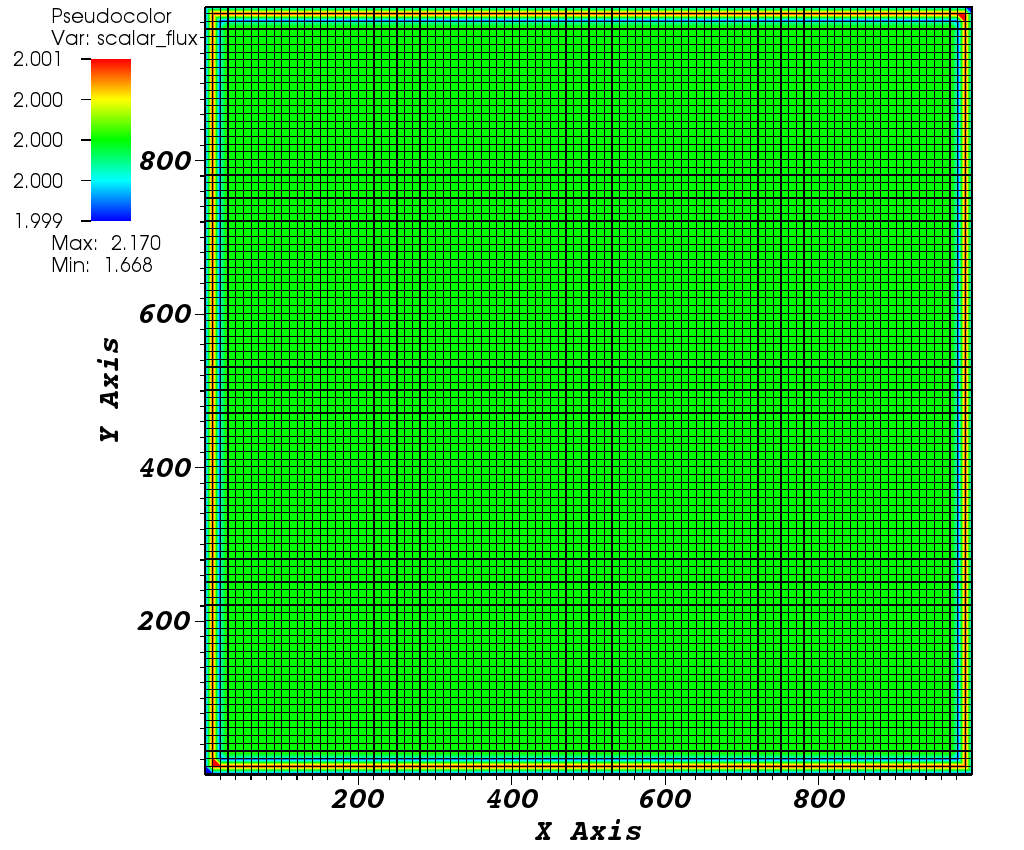
\includegraphics[width=0.63\textwidth]
  {./Janus/quad_diff}\label{quad_diff}}\\
  \subfloat[Quadrilateral cells]{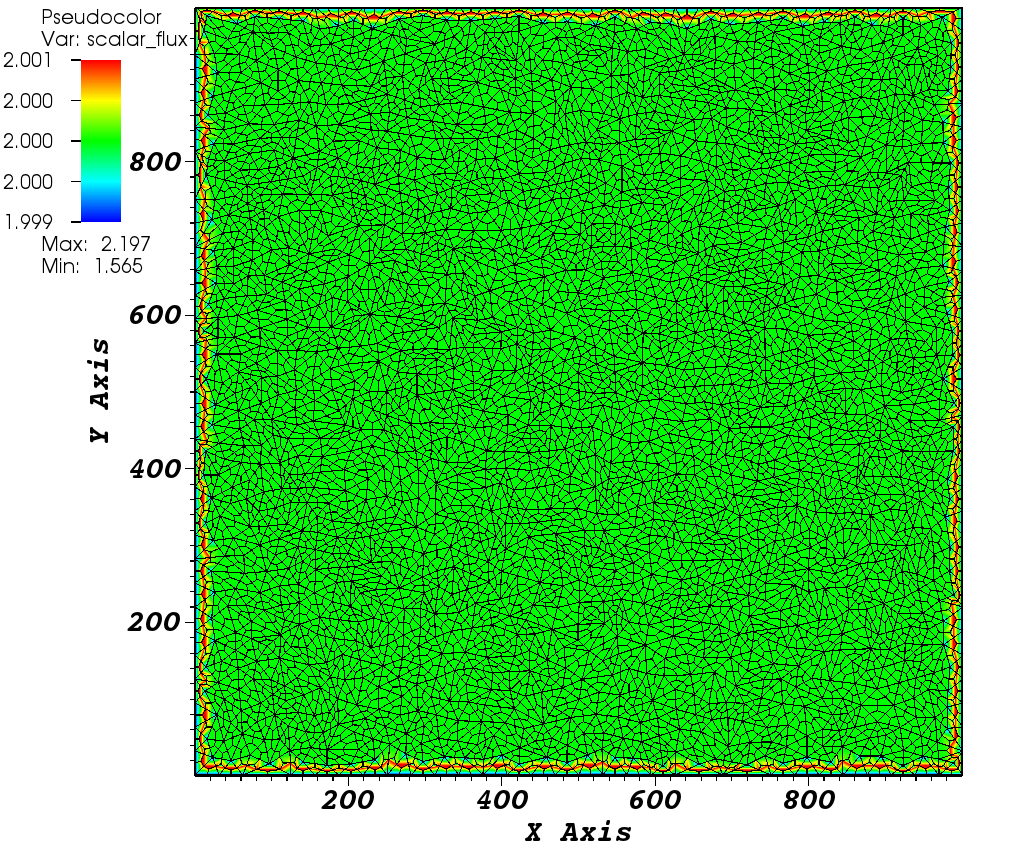
\includegraphics[width=0.63\textwidth]
  {./Janus/poly_diff}\label{poly_diff}}
  \caption{Scalar flux}
\end{figure}
\subsection{Convergence order}
In this test, we check the convergence order of PWLD and BLD on a benchmark.
We plot the error on average scalar fluxes as a function of the number of 
degrees of freedom. Since for two-dimensional geometries, the number of
degrees of freedom is
proportional to the square of the typical element size, the slopes of the 
graphs should equal one (PWLD and BLD are both second order methods). The test
that we chose is the IAEA EIR-2 benchmark problem \cite{Khalil1985}. This 
benchmark consists of five regions:
\begin{figure}[H]
  \centering
  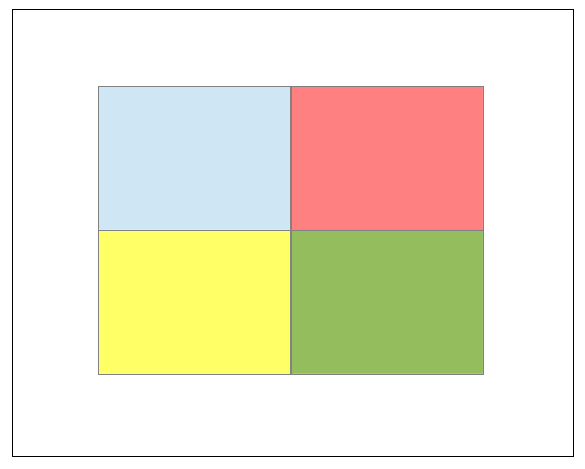
\includegraphics[width=0.4\textwidth]{./Janus/benchmark}
  \caption{Zones of the IAEA EIR-2 benchmark problem}
\end{figure}
The properties of the different zones are given in Table \ref{tabl_1}:
\begin{table}[H]
  \begin{center}
    \caption{Properties of the different zones of the benchmark}
    \begin{tabular}{|c|c|c|c|c|c|}
      \hline
    Zone & White & Blue & Salmon & Yellow & Green \\
      \hline
      Source $(n/(cm^3s))$ & 0    & 0    & 1    & 1    & 0 \\
    $\Sigma_t$ $(cm^{-1})$ & 0.9  & 0.65 & 0.7  & 0.6  & 0.48 \\
    $\Sigma_s$ $(cm^{-1})$ & 0.89 & 0.5  & 0.66 & 0.53 & 0.2 \\
             length ($cm$) & 96   & 30   & 30   & 30   & 30 \\
             height ($cm$) & 86   & 25   & 25   & 25   & 25 \\
      \hline
    \end{tabular}
    \label{tabl_1}
  \end{center}
\end{table}
The colored zones are in the middle of the white zone. In Figures \ref{glc_bld} 
and \ref{glc_pwld}, we show the convergence of the average scalar flux in the
different zones for $S_8$ Gauss-Legendre-Chebyshev quadrature when BLD and PWLD 
finite elements are used.
\begin{figure}[H]
  \centering
  \subfloat[BLD finite elements]{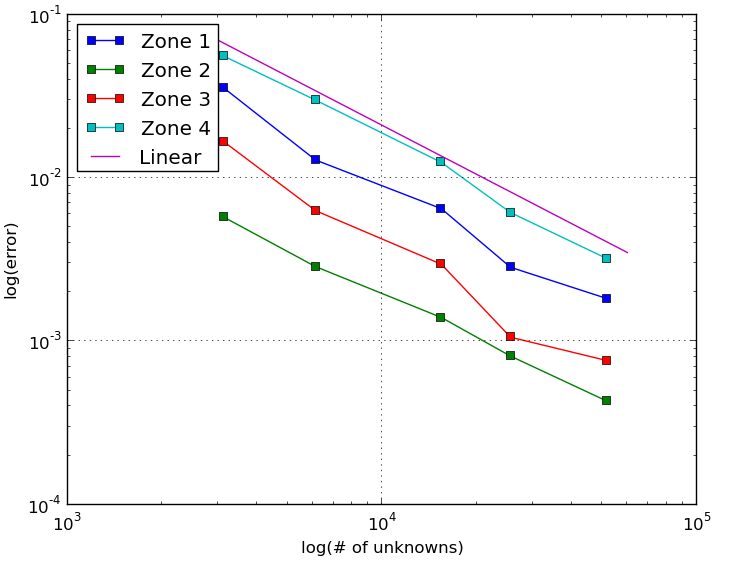
\includegraphics[width=0.5\textwidth]
  {./Janus/glc_conv_bld}\label{glc_bld}}
  \subfloat[PWLD finite elements]{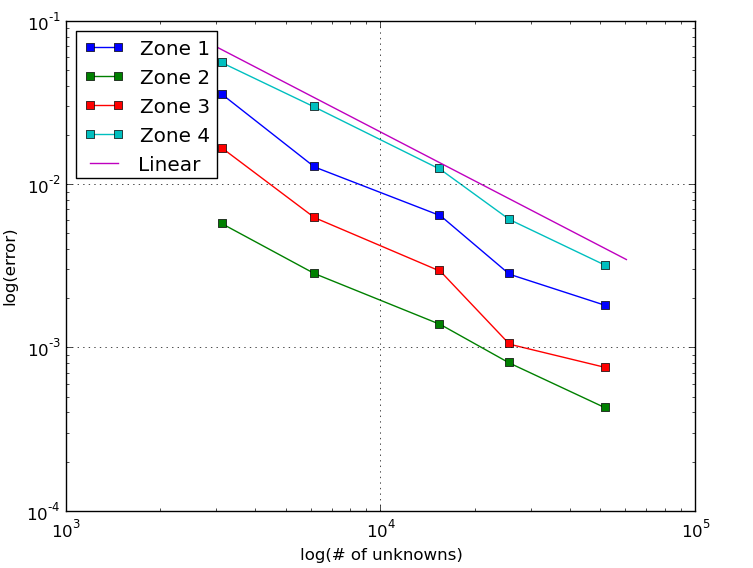
\includegraphics[width=0.5\textwidth]
  {./Janus/glc_conv_pwld}\label{glc_pwld}}
  \caption{Convergence of BLD and PWLD}
\end{figure}
We can see that the curves in all the zones have the right slope, i.e.,
the right order of convergence.
